\chapter{Keperiodikan}\label{ch:b1:periodicity}

Litium, natrium, dan kalium adalah logam lunak dan mengilap yang menjadi
kusam di udara dan bereaksi dengan air; fluorin, klor, dan brom adalah
nonlogam berwarna dan korosif yang merebut elektron dari hampir apa saja.
Setiap trio itu menempati satu kolom tabel periodik, dan anggota-anggota
satu kolom saling mirip, sedangkan tetangga sebaris tidak. Bab sebelumnya
menjelaskan sebabnya: unsur-unsur satu kolom mempunyai \omterm{def:b1:quantum-numbers:configuration}{konfigurasi
elektron} valensi yang sama. Bab ini mengubah penjelasan itu menjadi
angka --- jari-jari, energi ionisasi, \omterm{def:b1:periodicity:electron-affinity}{afinitas elektron},
\omterm{def:b1:periodicity:electronegativity}{keelektronegatifan} --- dan menjadi kecenderungan-kecenderungan yang
memungkinkan ahli kimia meramalkan, hanya dari letak sebuah unsur,
seberapa besar atom-atomnya, seberapa mudah atom itu melepas atau
menerima elektron, dan ke arah mana elektron-elektron sebuah ikatan
condong.

\begin{recall}
Setiap \omterm{def:b1:periodicity:table}{periode} dimulai dengan pengisian \omterm{def:b1:quantum-numbers:orbital}{subkulit} $n$s dan berakhir dengan
\omterm{def:b1:quantum-numbers:orbital}{subkulit} $n$p yang penuh; \omterm{def:b1:periodicity:table}{blok} s, p, d, dan f mempunyai lebar 2, 6, 10,
dan 14 (\cref{prop:b1:quantum-numbers:table}). Buku 1 (kelas 11)
memerikan \omterm{def:b1:periodicity:electronegativity}{keelektronegatifan} sebagai kecenderungan sebuah atom untuk
menarik elektron-elektron sebuah ikatan.
\end{recall}

\section{Tabel yang disusun dari konfigurasi}

\begin{definition}[Periode, golongan, blok]\label{def:b1:periodicity:table}
Dalam tabel periodik, unsur-unsur disusun menurut nomor atom $Z$ yang
membesar. Sebuah \emph{periode}\index{periode} adalah sebuah baris:
unsur-unsur yang kulit valensinya mempunyai bilangan utama $n$ yang sama.
Sebuah \emph{golongan}\index{golongan} adalah sebuah kolom, bernomor 1
sampai 18: unsur-unsur dengan konfigurasi valensi yang sama. Sebuah
\emph{blok}\index{blok} adalah himpunan unsur yang \omterm{def:b1:quantum-numbers:orbital}{subkulit} terakhirnya
yang terisi berjenis sama, s, p, d, atau f.
\end{definition}

\begin{example}[Membaca sebuah letak]\label{ex:b1:periodicity:position}
Selenium, $[\ce{Ar}]\,3\text{d}^{10} 4\text{s}^2 4\text{p}^4$, terletak
pada \omterm{def:b1:periodicity:table}{periode} 4 (kulit valensi $n = 4$), di \omterm{def:b1:periodicity:table}{blok} p, dan pada \omterm{def:b1:periodicity:table}{golongan} 16
(dua elektron s, sepuluh d, dan empat p: $2 + 10 + 4$); konfigurasi
valensinya, $n\text{s}^2 n\text{p}^4$, sama dengan konfigurasi oksigen
dan belerang di atasnya.
\end{example}

\begin{definition}[Logam, nonlogam, metaloid]\label{def:b1:periodicity:metalloid}
Logam adalah unsur yang padatannya menghantarkan listrik dan yang
atom-atomnya mudah melepas elektron membentuk kation; nonlogam adalah
unsur yang tidak menghantarkan listrik (dengan pengecualian seperti
grafit) dan mudah menerima elektron atau memakainya bersama. Sebuah
\emph{metaloid}\index{metaloid} adalah unsur yang sifatnya di antara
keduanya, yaitu semikonduktor: boron, silikon, germanium, arsen,
antimon, dan telurium.
\end{definition}

\begin{omfigure}
\omperiodictable[colour=metals, legend, f block=false]

{\small Logam (bagian terbesar), \omterm{def:b1:periodicity:metalloid}{metaloid} di sepanjang sebuah tangga dari
boron sampai telurium, dan nonlogam di kanan atas. \omterm{def:b1:periodicity:table}{Blok} f, yang tidak
digambar di sini, seluruhnya terdiri atas logam.}
\end{omfigure}

\section{Ukuran: jari-jari atom dan jari-jari ion}

\begin{definition}[Penapisan, muatan inti efektif]\label{def:b1:periodicity:screening}
Di dalam atom berelektron banyak, sebuah elektron ditarik oleh inti, yang
bermuatan $Ze$, dan ditolak oleh elektron-elektron lain. Elektron-elektron
bagian dalam sebagian meniadakan tarikan inti: inilah yang disebut
\emph{penapisan}\index{penapisan}. \omterm{def:b1:quantum-numbers:configuration}{Elektron valensi} berperilaku
seakan-akan merasakan muatan inti yang berkurang, $Z^{*}e$, yaitu
\emph{muatan inti efektif}\index{muatan inti efektif}, dengan
$Z^{*} < Z$. Elektron pada kulit yang lebih dalam menapis hampir
sepenuhnya; elektron pada kulit yang sama hanya sedikit menapis.
\end{definition}

\begin{remark}[Alat kualitatif]\label{rem:b1:periodicity:slater}
Dalam buku ini $Z^{*}$ dipakai secara kualitatif: sepanjang satu
\omterm{def:b1:periodicity:table}{periode}, $Z$ bertambah satu pada setiap langkah, sedangkan elektron
tambahannya, yang berada pada kulit yang sama, hanya sedikit menapis,
sehingga $Z^{*}$ yang dirasakan \omterm{def:b1:quantum-numbers:configuration}{elektron valensi} bertambah; menuruni satu
\omterm{def:b1:periodicity:table}{golongan}, $Z^{*}$ hanya sedikit berubah, tetapi kulit valensi $n$
bertambah. Aturan untuk menghitung $Z^{*}$ dari konfigurasi (aturan
Slater) diberikan dalam jilid Tahun 2.
\end{remark}

\begin{definition}[Jari-jari kovalen, jari-jari ion]\label{def:b1:periodicity:radius}
\emph{Jari-jari kovalen}\index{jari-jari kovalen} sebuah unsur adalah
setengah panjang ikatan tunggal antara dua atomnya: untuk klor, setengah
jarak \ce{Cl-Cl} pada \ce{Cl2}. \emph{Jari-jari ion}\index{jari-jari ion}
sebuah ion adalah bagian jarak antara kation dan anion yang bertetangga
di dalam kristal ion yang diberikan kepada ion itu, menurut sebuah
konvensi yang menetapkan jari-jari satu ion acuan (\ce{O^{2-}}); nilainya
sedikit bergantung pada banyaknya tetangga.
\end{definition}

\begin{example}[Halogen]\label{ex:b1:periodicity:halogen-radii}
Panjang ikatan \ce{F2}, \ce{Cl2}, \ce{Br2}, dan \ce{I2} adalah 141.2,
198.8, 228.1, dan \qty{266.6}{pm}, sehingga \omterm{def:b1:periodicity:radius}{jari-jari kovalennya} 71, 99,
114, dan \qty{133}{pm}: setiap langkah menuruni \omterm{def:b1:periodicity:table}{golongan} menambah satu
kulit dan sekitar \qty{20}{pm} atau lebih.
% ledger: re:F2, re:Cl2, re:Br2, re:I2
\end{example}

\begin{proposition}[Kecenderungan jari-jari]\label{prop:b1:periodicity:radius-trend}
Jari-jari atom mengecil dari kiri ke kanan sepanjang satu \omterm{def:b1:periodicity:table}{periode} dan
membesar dari atas ke bawah menuruni satu \omterm{def:b1:periodicity:table}{golongan}. Kation lebih kecil
daripada atomnya, anion lebih besar; dalam deret isoelektronik (ion-ion
dengan konfigurasi yang sama) jari-jari mengecil ketika $Z$ membesar.
\end{proposition}

\begin{proof}[Penalaran]
Ukuran atom adalah ukuran orbital-orbital valensinya, yang menyusut
ketika $Z^{*}$ membesar dan mengembang ketika $n$ membesar. Sepanjang
satu \omterm{def:b1:periodicity:table}{periode} $n$ tetap dan $Z^{*}$ membesar: atom-atomnya menyusut.
Menuruni satu \omterm{def:b1:periodicity:table}{golongan} $n$ bertambah satu pada setiap langkah, dan ini
mengalahkan perubahan kecil $Z^{*}$. Kation telah kehilangan kulit
valensinya, atau elektron-elektron yang saling tolak; anion telah
menerima satu elektron yang menolak elektron-elektron lainnya. Dalam
deret isoelektronik, elektron-elektron yang sama diikat oleh inti yang
muatannya makin besar.
\end{proof}

\begin{omfigure}
\begin{tikzpicture}[font=\small, x=1pt, y=1pt]
  % ledger: rion:O2-VI, rion:F-VI, rion:Na+VI, rion:Mg2+VI, rion:Al3+VI
  % radii in pm drawn at 0.30 pt per pm (circles to scale)
  \foreach \x/\r/\lab/\v in {40/140/\ce{O^{2-}}/140, 130/133/\ce{F-}/133,
      210/102/\ce{Na+}/102, 275/72/\ce{Mg^{2+}}/72, 325/53.5/\ce{Al^{3+}}/54} {
    \draw[fill=omDef!20, draw=omDef!70!black] (\x,0) circle ({0.30*\r});
    \node at (\x,0) {\lab};
    \node[below] at (\x,-50) {\v\,pm};
  }
  \node[anchor=west, align=left] at (350,0) {sepuluh elektron\\setiap ion,\\$Z = 8 \to 13$};
\end{tikzpicture}

{\small Deret isoelektronik $1\text{s}^2 2\text{s}^2 2\text{p}^6$,
digambar dengan skala sebenarnya (\omterm{def:b1:periodicity:radius}{jari-jari ion} untuk enam tetangga).
Kesepuluh elektron yang sama menyusut seiring bertambahnya muatan inti.}
\end{omfigure}

\section{Energi: ionisasi dan afinitas elektron}

\begin{definition}[Energi ionisasi]\label{def:b1:periodicity:ionisation-energy}
\emph{Energi ionisasi pertama}\index{energi ionisasi pertama} $E_{i1}$
sebuah unsur adalah energi yang diperlukan untuk melepaskan satu elektron
dari atom terisolasi dalam \omterm{def:b1:quantum-numbers:energy-level}{keadaan dasarnya}, dalam fase gas:
\[
  \ce{X(g) -> X+(g) + e-}, \qquad E_{i1} = E(\ce{X+}) + E(\ce{e-}) - E(\ce{X}) > 0 .
\]
\emph{Energi ionisasi berturut-turut}\index{energi ionisasi berturut-turut}
$E_{i2}, E_{i3}, \dots$ melepaskan elektron kedua, ketiga\dots\ dari
\ce{X+}, \ce{X^{2+}}\dots\ Nilainya dinyatakan dalam elektronvolt per
atom atau dalam kilojoule per mol
($\qty{1}{eV} \leftrightarrow \qty{96.49}{kJ/mol}$).
% ledger: const:NA, const:e (1 eV x N_A = 96.485 kJ/mol)
\end{definition}

\begin{omfigure}
\begin{tikzpicture}
\begin{axis}[
  width=0.92\linewidth, height=6.4cm,
  xmin=0, xmax=37, ymin=0, ymax=27,
  axis x line=bottom, axis y line=left,
  xlabel={nomor atom $Z$}, ylabel={$E_{i1}$ (eV)},
  xtick={2,10,18,36}, ytick={0,5,10,15,20,25},
  tick label style={font=\small}, label style={font=\small},
  clip=false]
\addplot[omDef, thick, mark=*, mark size=1.3pt] table[x=Z, y=IE_eV] {figdata/out/bachelor-1-ionisation-energies.dat};
\node[font=\small, anchor=south] at (axis cs:2,24.6) {He};
\node[font=\small, anchor=south] at (axis cs:10,21.6) {Ne};
\node[font=\small, anchor=south] at (axis cs:18,15.8) {Ar};
\node[font=\small, anchor=south] at (axis cs:36,14.0) {Kr};
\node[font=\small, anchor=north] at (axis cs:3,5.2) {Li};
\node[font=\small, anchor=north] at (axis cs:11,4.9) {Na};
\node[font=\small, anchor=north] at (axis cs:19,4.1) {K};
\node[font=\small, anchor=north] at (axis cs:31,5.8) {Ga};
\node[font=\small, anchor=north] at (axis cs:5,7.9) {B};
\node[font=\small, anchor=north] at (axis cs:8,13.2) {O};
\node[font=\small, anchor=north west] at (axis cs:13.1,6.0) {Al};
\node[font=\small, anchor=north] at (axis cs:16,9.9) {S};
\node[font=\small, anchor=south] at (axis cs:26,8.0) {logam 3d};
\end{axis}
\end{tikzpicture}

{\small \omterm{def:b1:periodicity:ionisation-energy}{Energi ionisasi pertama} 36 unsur pertama. Maksimum pada gas mulia,
minimum pada logam alkali; lekukan-lekukan kecil pada B, Al, Ga dan pada
O, S adalah efek \omterm{def:b1:quantum-numbers:orbital}{subkulit} pada
\cref{prop:b1:periodicity:ie-anomalies}.}
\end{omfigure}

\begin{proposition}[Kecenderungan energi ionisasi]\label{prop:b1:periodicity:ie-trend}
\omterm{def:b1:periodicity:ionisation-energy}{Energi ionisasi pertama} bertambah sepanjang satu \omterm{def:b1:periodicity:table}{periode}, dari logam
alkali sampai gas mulia, dan berkurang menuruni satu \omterm{def:b1:periodicity:table}{golongan}. \omterm{def:b1:periodicity:ionisation-energy}{Energi
ionisasi berturut-turut} selalu bertambah, $E_{i1} < E_{i2} < \dots$, dan
melonjak dengan faktor yang besar ketika elektron yang dilepaskan
berasal dari kulit yang lebih dalam.
\end{proposition}

\begin{proof}[Penalaran]
Melepaskan sebuah elektron lebih mudah jika elektron itu jauh dari inti
dan merasakan $Z^{*}$ yang kecil: sepanjang satu \omterm{def:b1:periodicity:table}{periode} $Z^{*}$ membesar
dan jari-jari menyusut; menuruni satu \omterm{def:b1:periodicity:table}{golongan} jari-jari membesar. Setiap
elektron berikutnya ditarik dari ion yang muatannya lebih besar dan
ukurannya lebih kecil, sehingga lebih mahal; begitu kulit valensi kosong,
elektron berikutnya berasal dari kulit dengan $n$ yang lebih kecil, jauh
lebih dekat ke inti dan hampir tidak tertapis sama sekali.
\end{proof}

\begin{example}[Magnesium]\label{ex:b1:periodicity:magnesium}
\omterm{def:b1:periodicity:ionisation-energy}{Energi ionisasi berturut-turut} magnesium adalah 7.65, 15.04, 80.14, dan
\qty{109.27}{eV}. Rasio $E_{i2}/E_{i1} \approx 2$ masih sedang;
$E_{i3}/E_{i2} \approx 5.3$ adalah sebuah lonjakan: elektron ketiga
berasal dari teras 2p. Magnesium melepaskan kedua elektron 3s-nya dan
berhenti pada \ce{Mg^{2+}}, yang berkonfigurasi gas mulia neon.
% ledger: ie:Mg, ie2:Mg, ie3:Mg, ie4:Mg
\end{example}

\begin{omfigure}
\begin{tikzpicture}
\begin{axis}[
  width=0.55\linewidth, height=5.2cm, ybar, bar width=14pt,
  xmin=0.4, xmax=4.6, ymin=1, ymax=300, ymode=log,
  axis x line=bottom, axis y line=left,
  xlabel={elektron yang dilepas}, ylabel={$E_{i}$ (eV)},
  xtick={1,2,3,4}, xticklabels={ke-1,ke-2,ke-3,ke-4},
  tick label style={font=\small}, label style={font=\small},
  nodes near coords={\pgfmathprintnumber[fixed, fixed zerofill, precision=2]{\pgfplotspointmeta}},
  nodes near coords style={font=\scriptsize},
  point meta=rawy]
\addplot[fill=omDef!40, draw=omDef] table[x=k, y=IE_eV] {figdata/out/bachelor-1-ionisation-energies-mg.dat};
\end{axis}
\end{tikzpicture}

{\small \omterm{def:b1:periodicity:ionisation-energy}{Energi ionisasi berturut-turut} magnesium (sumbu logaritmik).
Energi ketiga lima kali energi kedua: kulit 3s sudah kosong dan teras
tercapai.}
\end{omfigure}

\begin{proposition}[Dua lekukan sepanjang periode]\label{prop:b1:periodicity:ie-anomalies}
Sepanjang \omterm{def:b1:periodicity:table}{periode} 2 dan 3, \omterm{def:b1:periodicity:ionisation-energy}{energi ionisasi pertama} sedikit turun dari
\omterm{def:b1:periodicity:table}{golongan} 2 ke \omterm{def:b1:periodicity:table}{golongan} 13 (\ce{Be} ke \ce{B}, \ce{Mg} ke \ce{Al}) dan
dari \omterm{def:b1:periodicity:table}{golongan} 15 ke \omterm{def:b1:periodicity:table}{golongan} 16 (\ce{N} ke \ce{O}, \ce{P} ke \ce{S}).
\end{proposition}

\begin{proof}[Penalaran]
Pada \ce{B} dan \ce{Al}, elektron yang dilepaskan adalah elektron p
pertama, yang energinya lebih tinggi daripada elektron s pada \ce{Be}
dan \ce{Mg}. Pada \ce{O} dan \ce{S}, elektron yang dilepaskan adalah
elektron p keempat, yang pertama berbagi orbital (\omorbs{ud,u,u}):
tolakannya dengan pasangannya membuatnya lebih mudah dilepaskan daripada
elektron \omterm{def:b1:quantum-numbers:orbital}{subkulit} setengah penuh pada \ce{N} atau \ce{P}
(\omorbs{u,u,u}).
% ledger: ie:Be, ie:B, ie:N, ie:O, ie:Mg, ie:Al, ie:P, ie:S
\end{proof}

\begin{definition}[Afinitas elektron]\label{def:b1:periodicity:electron-affinity}
\emph{Afinitas elektron}\index{afinitas elektron} $E_{ea}$ sebuah unsur
adalah energi yang dilepaskan ketika sebuah atom terisolasi dalam
\omterm{def:b1:quantum-numbers:energy-level}{keadaan dasarnya} menangkap sebuah elektron dalam fase gas,
\[
  \ce{X(g) + e- -> X-(g)}, \qquad E_{ea} = E(\ce{X}) + E(\ce{e-}) - E(\ce{X-}) .
\]
Nilainya positif jika anion lebih stabil daripada atom beserta elektron
bebasnya.
\end{definition}

\begin{example}[Halogen dan tetangga-tetangganya]\label{ex:b1:periodicity:ea}
\omterm{def:b1:periodicity:electron-affinity}{Afinitas elektron} \ce{F}, \ce{Cl}, \ce{Br}, dan \ce{I} adalah 3.40, 3.61,
3.36, dan \qty{3.06}{eV}, yang terbesar di antara semua unsur; afinitas
\ce{O} dan \ce{S} adalah 1.44 dan \qty{2.02}{eV}, \ce{C} \qty{1.26}{eV},
\ce{Na} \qty{0.55}{eV}. Atom yang melengkapi sebuah \omterm{def:b1:quantum-numbers:orbital}{subkulit} dengan
menangkap satu elektron (halogen) melepaskan banyak energi. Nitrogen,
berilium, magnesium, dan gas mulia tidak membentuk anion gas yang stabil:
elektron tambahannya harus berpasangan di dalam \omterm{def:b1:quantum-numbers:orbital}{subkulit} p yang setengah
penuh atau memasuki \omterm{def:b1:quantum-numbers:orbital}{subkulit} baru. Afinitas fluorin lebih kecil daripada
afinitas klor karena elektron tambahannya berdesakan di dalam kulit 2p
yang kecil.
% ledger: ea:F, ea:Cl, ea:Br, ea:I, ea:O, ea:S, ea:C, ea:Na
\end{example}

\section{Keelektronegatifan dan polarisabilitas}

\begin{definition}[Keelektronegatifan]\label{def:b1:periodicity:electronegativity}
\emph{Keelektronegatifan}\index{keelektronegatifan} $\chi$ sebuah unsur
mengukur kecenderungan atom-atomnya, di dalam molekul, untuk menarik
elektron-elektron ikatan yang dibentuknya. Ada dua skala yang dipakai.
\begin{itemize}
  \item Pada \emph{skala Pauling}\index{skala Pauling}, selisihnya
        didefinisikan dari energi ikatan $D$:
        \[
          |\chi_A - \chi_B| = \sqrt{\frac{\Delta E}{\qty{1}{eV}}}, \qquad
          \Delta E = D(\text{A--B}) - \tfrac12\big[D(\text{A--A}) +
          D(\text{B--B})\big],
        \]
        dan skala ini ditambatkan pada $\chi(\ce{F}) = 3.98$.
  \item Pada \emph{skala Mulliken}\index{skala Mulliken},
        $\chi_M = \tfrac12\,(E_{i1} + E_{ea})$, dalam elektronvolt.
\end{itemize}
\end{definition}

\begin{remark}[Mengapa ada kelebihan energi ikatan]\label{rem:b1:periodicity:pauling}
Seandainya kedua atom ikatan A--B menarik elektron-elektronnya sama kuat,
energi ikatannya kira-kira sama dengan rata-rata energi ikatan A--A dan
B--B. Jika satu atom lebih elektronegatif, ikatan itu memperoleh sifat
ion parsial, $\ce{A^{\delta+}-B^{\delta-}}$, yang tarikan
elektrostatiknya menambah energi: $\Delta E > 0$ mengukur ketidakmerataan
pemakaian bersama itu. Definisi Mulliken mengatakan hal yang sama dari
sisi atom: atom yang mengikat elektronnya sendiri dengan kuat ($E_i$
besar) dan menyambut elektron tambahan ($E_{ea}$ besar) menarik
elektron-elektron sebuah ikatan.
\end{remark}

\begin{omfigure}
% ledger: en:H, en:Li, en:Be, en:B, en:C, en:N, en:O, en:F, en:Na, en:Mg,
% en:Al, en:Si, en:P, en:S, en:Cl, en:K, en:Ca, en:Ga, en:Ge, en:As, en:Se,
% en:Br, en:Rb, en:Sr, en:In, en:Sn, en:Sb, en:Te, en:I, en:Cs, en:Ba
\omperiodictable[upto=56, f block=false, numbers=false, highlight colour=omDef!12,
  highlight={F,O,N,Cl}, values={H/2.20,Li/0.98,Be/1.57,B/2.04,C/2.55,N/3.04,O/3.44,F/3.98,
  Na/0.93,Mg/1.31,Al/1.61,Si/1.90,P/2.19,S/2.58,Cl/3.16,K/0.82,Ca/1.00,Ga/1.81,Ge/2.01,
  As/2.18,Se/2.55,Br/2.96,Rb/0.82,Sr/0.95,In/1.78,Sn/1.96,Sb/2.05,Te/2.10,I/2.66,
  Cs/0.79,Ba/0.89}]

{\small \omterm{def:b1:periodicity:electronegativity}{Keelektronegatifan} Pauling unsur-unsur \omterm{def:b1:periodicity:table}{golongan} utama (\omterm{def:b1:periodicity:table}{blok} d
dibiarkan kosong). Nilainya bertambah dari kiri ke kanan dan dari bawah
ke atas; keempat unsur yang paling elektronegatif, F, O, Cl, dan N,
diarsir.}
\end{omfigure}

\begin{proposition}[Kecenderungan keelektronegatifan]\label{prop:b1:periodicity:en-trend}
\omterm{def:b1:periodicity:electronegativity}{Keelektronegatifan} bertambah sepanjang satu \omterm{def:b1:periodicity:table}{periode} dan berkurang
menuruni satu \omterm{def:b1:periodicity:table}{golongan}: fluorin adalah unsur yang paling elektronegatif,
sesium dan fransium yang paling tidak elektronegatif. Selisih
$\Delta\chi$ antara dua atom yang berikatan menentukan sifat ikatannya:
$\Delta\chi < 0.4$ kovalen yang hampir nonpolar,
$0.4 < \Delta\chi < 1.7$ kovalen polar, $\Delta\chi > 1.7$ terutama
ionik --- tiga daerah pada sebuah kesinambungan, bukan kelas-kelas yang
tegas.
\end{proposition}

\begin{example}[Tiga ikatan]\label{ex:b1:periodicity:bonds}
\ce{C-H}: $\Delta\chi = 2.55 - 2.20 = 0.35$, hampir nonpolar;
\ce{O-H}: $3.44 - 2.20 = 1.24$, polar, dengan oksigen membawa muatan
negatif parsial; \ce{Na-Cl}: $3.16 - 0.93 = 2.23$, ionik.
% ledger: en:C, en:H, en:O, en:Na, en:Cl
\end{example}

\begin{definition}[Polarisabilitas]\label{def:b1:periodicity:polarisability}
\emph{Polarisabilitas}\index{polarisabilitas} sebuah atom, ion, atau
molekul mengukur seberapa mudah awan elektronnya diubah bentuknya oleh
medan listrik --- medan ion atau dipol di dekatnya. Spesies yang mudah
terpolarisasi memperoleh, di dalam medan, momen dipol imbas yang
sebanding dengan kuat medan itu.
\end{definition}

\begin{proposition}[Kecenderungan polarisabilitas]\label{prop:b1:periodicity:polarisability-trend}
\omterm{def:b1:periodicity:polarisability}{Polarisabilitas} membesar dengan ukuran awan elektron dan dengan
banyaknya elektron, serta mengecil dengan muatan inti yang mengikatnya:
\omterm{def:b1:periodicity:polarisability}{polarisabilitas} bertambah menuruni satu \omterm{def:b1:periodicity:table}{golongan} ($\ce{F-} < \ce{Cl-} < \ce{Br-} <
\ce{I-}$), anion jauh lebih mudah terpolarisasi daripada
kation, dan anion besar yang lunak seperti \ce{I-} adalah spesies umum
yang paling mudah terpolarisasi.
\end{proposition}

\begin{example}[Mengapa polarisabilitas penting]\label{ex:b1:periodicity:pol}
Gaya tarik London antarmolekul, pokok bahasan
\cref{ch:b1:intermolecular-forces-solvents}, membesar dengan
\omterm{def:b1:periodicity:polarisability}{polarisabilitas}: diiodin berwujud padat pada suhu kamar, sedangkan
diklor berwujud gas. Di dalam kristal ion, kation kecil yang bermuatan
besar memolarisasi anion yang besar dan memberi ikatannya sedikit sifat
kovalen, yaitu kegagalan model ion sederhana yang dijumpai pada
\cref{ch:b1:crystals-ionic-covalent}.
\end{example}

\begin{history}[Skala Pauling, 1932]
Pada tahun 1932 ahli kimia Amerika Linus Pauling memperhatikan bahwa
energi ikatan antara dua atom yang berbeda hampir selalu lebih besar
daripada rata-rata energi kedua ikatan simetrisnya, dan dari kelebihan
itu ia menyusun skala \omterm{def:b1:periodicity:electronegativity}{keelektronegatifan} yang pertama. Skalanya, yang
direvisi seiring diukurnya energi ikatan yang lebih baik, masih menjadi
skala yang tercantum dalam setiap tabel. Pauling menerima Hadiah Nobel
Kimia pada tahun 1954 untuk karyanya tentang ikatan kimia, dan Hadiah
Nobel Perdamaian pada tahun 1962.
\end{history}

\begin{omfigure}
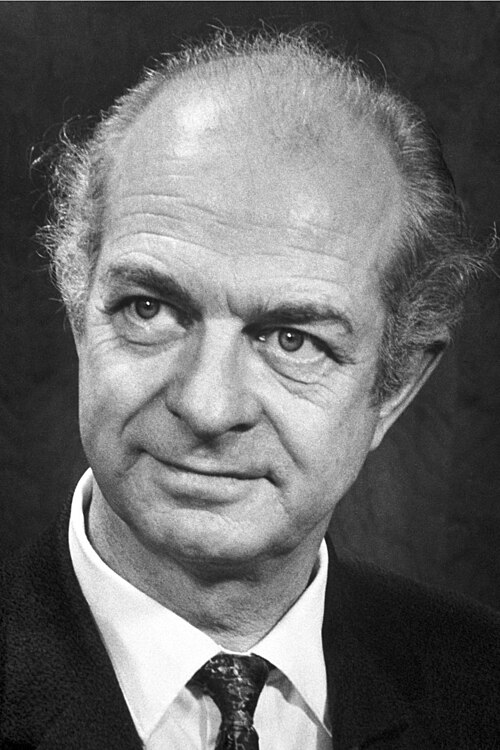
\includegraphics[width=0.24\linewidth]{images/book2/pauling.jpg}

{\small Linus Pauling (1901--1994).}
\end{omfigure}

\section{Kecenderungan sifat kimia}

\begin{proposition}[Sifat pereduksi dan sifat pengoksidasi]\label{prop:b1:periodicity:redox-trend}
Unsur-unsur yang energi ionisasi dan \omterm{def:b1:periodicity:electronegativity}{keelektronegatifannya} rendah, di
sebelah kiri tabel dan di bagian bawah \omterm{def:b1:periodicity:table}{golongannya}, mudah melepaskan
elektron: unsur-unsur itu adalah logam pereduksi (terutama logam
alkali). Unsur-unsur yang \omterm{def:b1:periodicity:electronegativity}{keelektronegatifan} dan \omterm{def:b1:periodicity:electron-affinity}{afinitas elektronnya}
tinggi, di kanan atas, mudah menerima elektron: unsur-unsur itu adalah
nonlogam pengoksidasi (terutama fluorin, oksigen, dan klor). Gas mulia,
yang energi ionisasinya tinggi dan tidak mempunyai afinitas terhadap
elektron tambahan, tidak melakukan keduanya.
\end{proposition}

\begin{method}[Meramalkan kecenderungan dari letak unsur]\label{met:b1:periodicity:predict}
Untuk membandingkan dua unsur dalam suatu sifat yang berkaitan dengan
kuatnya inti mengikat \omterm{def:b1:quantum-numbers:configuration}{elektron valensi} (jari-jari, $E_i$, $E_{ea}$,
$\chi$):
\begin{enumerate}
  \item jika keduanya segolongan, yang letaknya lebih bawah mempunyai $n$
        yang lebih besar: jari-jari lebih besar, $E_i$ dan $\chi$ lebih
        kecil;
  \item jika keduanya seperiode, yang letaknya lebih kanan mempunyai
        $Z^{*}$ yang lebih besar: jari-jari lebih kecil, $E_i$ dan $\chi$
        lebih besar;
  \item jika tidak, bandingkan masing-masing dengan unsur di persilangan
        barisnya dan kolom unsur yang lain;
  \item periksa efek \omterm{def:b1:quantum-numbers:orbital}{subkulit} (awal sebuah \omterm{def:b1:quantum-numbers:orbital}{subkulit} p, elektron p
        pertama yang berpasangan) sebelum menyimpulkan tentang energi
        ionisasi.
\end{enumerate}
\end{method}

\begin{example}[Litium dalam baterai]\label{ex:b1:periodicity:lithium}
Litium mempunyai \omterm{def:b1:periodicity:electronegativity}{keelektronegatifan} terendah di \omterm{def:b1:periodicity:table}{periode} 2 dan mudah
melepaskan elektron 2s-nya, sementara ia adalah logam yang paling ringan:
litium membawa muatan yang dapat dipindahkan per gram paling banyak di
antara semua unsur, itulah sebabnya ia menggerakkan baterai isi ulang.
\omterm{def:b1:periodicity:ionisation-energy}{Energi ionisasi pertamanya}, \qty{5.39}{eV}, lebih besar daripada energi
ionisasi natrium (5.14) atau kalium (4.34), tetapi di dalam air litium
adalah logam alkali yang paling pereduksi, sebuah paradoks yang
terpecahkan oleh hidrasi kuat ion \ce{Li+} yang kecil
(\cref{ch:b1:nernst}).
% ledger: ie:Li, ie:Na, ie:K
\end{example}

\section{Latihan}

\begin{exercise}[$\star$]\label{exo:b1:periodicity:1}
Tentukan \omterm{def:b1:periodicity:table}{periode}, \omterm{def:b1:periodicity:table}{golongan}, dan \omterm{def:b1:periodicity:table}{blok} kalsium, besi, selenium, dan iodin
($Z = 20, 26, 34, 53$) dari konfigurasinya.
\end{exercise}

\begin{exercise}[$\star$]\label{exo:b1:periodicity:2}
Pada setiap pasangan, spesies manakah yang lebih besar, dan mengapa?
\ce{Na} atau \ce{Cl}; \ce{Na} atau \ce{Na+}; \ce{F-} atau \ce{Cl-};
\ce{Na+} atau \ce{Mg^{2+}}.
\end{exercise}

\begin{exercise}[$\star$]\label{exo:b1:periodicity:3}
\omterm{def:b1:periodicity:ionisation-energy}{Energi ionisasi pertama} \ce{Na}, \ce{Mg}, \ce{Al}, \ce{P}, \ce{S}, dan
\ce{Ar} adalah 5.14, 7.65, 5.99, 10.49, 10.36, dan \qty{15.76}{eV}.
Urutkan nilai-nilai itu dan tunjukkan dua penyimpangan dari kecenderungan
umumnya.
\end{exercise}

\begin{exercise}[$\star$]\label{exo:b1:periodicity:4}
Definisikan \omterm{def:b1:periodicity:polarisability}{polarisabilitas} sebuah spesies. Manakah yang lebih mudah
terpolarisasi, \ce{F-} atau \ce{I-}? \ce{Na+} atau \ce{Cl-}? Berikan
alasannya.
\end{exercise}

\begin{exercise}[$\star\star$]\label{exo:b1:periodicity:5}
Keempat \omterm{def:b1:periodicity:ionisation-energy}{energi ionisasi pertama} sebuah unsur \omterm{def:b1:periodicity:table}{periode} 3 adalah 5.99,
18.83, 28.45, dan \qty{119.99}{eV}. Hitunglah rasio-rasio berturut-turutnya,
lalu tentukan unsur itu dan ion yang dibentuknya.
\end{exercise}

\begin{exercise}[$\star\star$]\label{exo:b1:periodicity:6}
Jelaskan mengapa klor mempunyai \omterm{def:b1:periodicity:electron-affinity}{afinitas elektron} yang lebih besar
daripada fluorin, dan mengapa nitrogen dan magnesium tidak membentuk anion
gas yang stabil.
\end{exercise}

\begin{exercise}[$\star\star$]\label{exo:b1:periodicity:7}
Hitunglah \omterm{def:b1:periodicity:electronegativity}{keelektronegatifan} Mulliken natrium ($E_{i1} =
\qty{5.14}{eV}$, $E_{ea} = \qty{0.55}{eV}$) dan klor ($E_{i1} =
\qty{12.97}{eV}$, $E_{ea} = \qty{3.61}{eV}$). Apa yang ditunjukkan
nilai-nilai itu tentang ikatan dalam \ce{NaCl}?
\end{exercise}

\begin{exercise}[$\star\star$]\label{exo:b1:periodicity:8}
Dengan nilai Pauling pada \cref{ex:b1:periodicity:bonds} dan $\chi(\ce{F})
= 3.98$, golongkan ikatan \ce{H-F}, \ce{C-H}, \ce{Na-Cl}, \ce{C-Cl}
($\chi(\ce{Cl}) = 3.16$), dan \ce{O-H}, lalu tentukan tanda muatan parsial
pada setiap atom.
\end{exercise}

\begin{exercise}[$\star\star$]\label{exo:b1:periodicity:9}
\omterm{def:b1:periodicity:ionisation-energy}{Energi ionisasi pertama} \ce{Li}, \ce{Na}, dan \ce{K} adalah 5.39, 5.14,
dan \qty{4.34}{eV}. Jelaskan kecenderungan itu dan ramalkan apakah \omterm{def:b1:periodicity:ionisation-energy}{energi
ionisasi pertama} rubidium di atas atau di bawah \qty{4.34}{eV}.
\end{exercise}

\begin{exercise}[$\star\star\star$]\label{exo:b1:periodicity:10}
Seng ($Z = 30$) mempunyai \omterm{def:b1:periodicity:ionisation-energy}{energi ionisasi pertama} \qty{9.39}{eV} dan
galium ($Z = 31$) \qty{6.00}{eV}; arsen ($Z = 33$) \qty{9.79}{eV} dan
selenium ($Z = 34$) \qty{9.75}{eV}. Jelaskan kedua penurunan itu dengan
menggunakan konfigurasinya.
\end{exercise}

\begin{exercise}[$\star\star\star$]\label{exo:b1:periodicity:11}
Ambil $D(\ce{H-H}) = \qty{436}{kJ/mol}$, $D(\ce{F-F}) =
\qty{158}{kJ/mol}$, $\chi(\ce{H}) = 2.20$, dan $\chi(\ce{F}) = 3.98$,
dengan $\qty{1}{eV} = \qty{96.5}{kJ/mol}$. Gunakan definisi Pauling untuk
memperkirakan energi ikatan $D(\ce{H-F})$. Mengapa nilainya jauh lebih
besar daripada rata-rata kedua ikatan simetris?
\end{exercise}

\begin{exercise}[$\star\star\star$]\label{exo:b1:periodicity:12}
\omterm{def:b1:periodicity:electronegativity}{Keelektronegatifan} Pauling ditabelkan untuk kripton (3.00) dan xenon
(2.60), tetapi tidak untuk helium, neon, atau argon. Dengan definisi
skala itu, jelaskan mengapa sebuah nilai hanya dapat diberikan untuk
unsur yang membentuk ikatan, dan mengapa gas mulia yang lebih berat yang
membentuk ikatan.
% ledger: en:Kr, en:Xe
\end{exercise}

\section{Soal: Aritmetika Pauling}

\begin{problem}[{Soal akhir pekan --- sebuah unsur tak dikenal dari
energi ionisasinya, sederet ion dengan awan elektron yang sama, dua
skala keelektronegatifan, dan angka Pauling untuk ikatan H--Cl}]
\label{pb:b1:periodicity:1}
Data: $\qty{1}{eV}$ per partikel setara dengan \qty{96.485}{kJ/mol}.

\medskip
\noindent\textbf{Bagian I --- Sebuah unsur tak dikenal.}
Keempat \omterm{def:b1:periodicity:ionisation-energy}{energi ionisasi pertama} sebuah unsur X \omterm{def:b1:periodicity:table}{periode} 3 adalah 7.65,
15.04, 80.14, dan \qty{109.27}{eV}.
\begin{enumerate}
  \item Mengapa setiap energi ionisasi lebih besar daripada yang
        sebelumnya?
  \item Hitunglah rasio $E_{i2}/E_{i1}$, $E_{i3}/E_{i2}$, dan
        $E_{i4}/E_{i3}$.
  \item Turunkan \omterm{def:b1:periodicity:table}{golongan} X, lalu tentukan unsur itu.
  \item Ion apakah yang dibentuk X dalam senyawa-senyawanya? Tuliskan
        konfigurasinya.
  \item Apakah X logam atau nonlogam? Berikan alasan dari letaknya.
  \item Mengapa elektron ketiga jauh lebih mahal daripada elektron kedua?
\end{enumerate}

\medskip
\noindent\textbf{Bagian II --- Sepuluh elektron.}
\omterm{def:b1:periodicity:radius}{Jari-jari ion} (enam tetangga) \ce{O^{2-}}, \ce{F-}, \ce{Na+},
\ce{Mg^{2+}}, dan \ce{Al^{3+}} adalah 140, 133, 102, 72, dan
\qty{54}{pm}.
\begin{enumerate}[resume]
  \item Tunjukkan bahwa ion-ion ini mempunyai konfigurasi yang sama.
  \item Jelaskan urutan jari-jarinya.
  \item Manakah di antara kelima ion itu yang paling mudah
        terpolarisasi, dan mengapa?
  \item Hitunglah rasio jari-jari terbesar terhadap jari-jari terkecil.
  \item Panjang ikatan \ce{Cl2} adalah \qty{198.8}{pm} dan jari-jari
        \ce{Cl-} \qty{181}{pm}. Hitunglah \omterm{def:b1:periodicity:radius}{jari-jari kovalen} klor, lalu
        bandingkan.
  \item Tanpa data tambahan, urutkan \ce{Cl-}, \ce{Na+}, dan \ce{Mg^{2+}}
        menurut ukurannya.
\end{enumerate}

\medskip
\noindent\textbf{Bagian III --- \omterm{def:b1:periodicity:electronegativity}{Skala Mulliken}.}
\begin{center}
\small
\begin{tabular}{lccccc}
\hline
unsur & \ce{F} & \ce{Cl} & \ce{Br} & \ce{O} & \ce{C} \\
\hline
$E_{i1}$ (eV) & 17.42 & 12.97 & 11.81 & 13.62 & 11.26 \\
$E_{ea}$ (eV) & 3.40 & 3.61 & 3.36 & 1.44 & 1.26 \\
$\chi$ Pauling & 3.98 & 3.16 & 2.96 & 3.44 & 2.55 \\
\hline
\end{tabular}
\end{center}
% ledger: ie:F, ie:Cl, ie:Br, ie:O, ie:C, ea:F, ea:Cl, ea:Br, ea:O, ea:C,
% en:F, en:Cl, en:Br, en:O, en:C
\begin{enumerate}[resume]
  \item Hitunglah \omterm{def:b1:periodicity:electronegativity}{keelektronegatifan} Mulliken kelima unsur itu.
  \item Urutkan unsur-unsur itu pada setiap skala. Unsur manakah yang
        letaknya berbeda?
  \item Hitunglah rasio $\chi_{\text{Pauling}}/\chi_M$ untuk ketiga
        halogen. Apa yang tampak?
  \item Kemukakan mengapa oksigen menyimpang dari aturan halogen
        (perhatikan \omterm{def:b1:periodicity:electron-affinity}{afinitas elektronnya}).
  \item Atom manakah yang membawa muatan negatif parsial dalam \ce{HCl}?
        dalam \ce{ClF}?
  \item Dengan nilai-nilai dalam tabel ($\chi(\ce{H}) = 2.20$), apakah
        ikatan \ce{H-Cl} kovalen nonpolar, kovalen polar, atau ionik?
\end{enumerate}

\medskip
\noindent\textbf{Bagian IV --- Angka Pauling untuk H--Cl.}
Entalpi pembentukan standar \ce{H(g)}, \ce{Cl(g)}, dan \ce{HCl(g)} pada
\qty{298}{K} adalah 218.0, 121.3, dan \qty{-92.3}{kJ/mol}; entalpi
pembentukan \ce{H2(g)} dan \ce{Cl2(g)} sama dengan nol. Energi ikatan
sebuah molekul diambil sebagai entalpi disosiasinya menjadi atom-atom.
% ledger: janaf:H, janaf:Cl, janaf:HCl
\begin{enumerate}[resume]
  \item Hitunglah $D(\ce{H-H})$ dari \ce{H2(g) -> 2H(g)}.
  \item Hitunglah $D(\ce{Cl-Cl})$.
  \item Hitunglah $D(\ce{H-Cl})$ dari \ce{HCl(g) -> H(g) + Cl(g)}.
  \item Hitunglah kelebihan energi Pauling $\Delta E$ dalam kJ/mol, lalu
        tunjukkan bahwa nilainya sama dengan $-\Delta_f H(\ce{HCl})$.
  \item Ubahlah $\Delta E$ menjadi elektronvolt.
  \item Hitunglah $|\chi(\ce{Cl}) - \chi(\ce{H})|$, lalu bandingkan
        dengan selisih nilai-nilai dalam tabel, $3.16 - 2.20$.
\end{enumerate}
\end{problem}
